\documentclass[12pt,a4paper]{article}
\usepackage{amsmath,amssymb,fullpage,graphicx}
\let\hat\widehat
\let\tilde\widetilde

\usepackage{amssymb}
\usepackage{amsmath}
\usepackage{epsfig, graphics}
\usepackage{latexsym}
\usepackage{fullpage}
\usepackage{bm}
\usepackage[parfill]{parskip}
\usepackage{subfigure}
\usepackage{fixltx2e}
\usepackage{listings}

%%%% new version of enumerate with less spacing
\newenvironment{enum}{
\begin{enumerate}
  \setlength{\itemsep}{1pt}
  \setlength{\parskip}{0pt}
  \setlength{\parsep}{0pt}
}{\end{enumerate}}

% TODO : fill your custom commands here if needed
\newcommand{\Ab}{\bm{A}}

\begin{document}

\begin{center}
    {\bf\large Homework 1} \\
    {\bf\large M1522.001000 Computer Vision (2017 Spring)} \\
    2017-81517 Patric Steiner \\
    Date: March 9 Thursday
\end{center}

\textbf{[Important] Reference to work of others.} You can refer to another person's key idea in writing the source code, but in this case you must leave a reference in the writeup. If you take someone else's idea and leave a reference, you will only get 0 points in the "Implementation" part of that problem in the scoring process. 
However, please note that if you do not mention the reference even though you have brought in someone else's idea, you will get 0 points for all the problems in that homework.




%%%%%%%%%%%%%%%%%%%%%%%%%%%%%%%%%%%%%%%%%%%%%%
% Q1
%%%%%%%%%%%%%%%%%%%%%%%%%%%%%%%%%%%%%%%%%%%%%%
\section{Composing Filters [5 points]}

Yes, applying G followed by E is equivalent to applying E and then G, because they are both linear kernels and can be applied by convolution. Convolution is commutative and associative, so the order is irrelevant.
If M is used however, the result will not be the same. M is a median filter, so it is non-linear and thus cannot be applied using convolution. The result will vary depeding if E or M is applied first.

%%%%%%%%%%%%%%%%%%%%%%%%%%%%%%%%%%%%%%%%%%%%%%
% Q2
%%%%%%%%%%%%%%%%%%%%%%%%%%%%%%%%%%%%%%%%%%%%%%
\section{Decomposing a Steerable Filter [10 pts]}

A 2D gaussian filter is symmetrical and thus can be separated into two 1D gaussian (horizontal and vertical) filters:
\begin{equation}
    G(x,y) = \frac{1}{2\pi\sigma^2} exp(-\frac{x^2+y^2}{2\sigma^2}) \\
    = \frac{1}{2\pi\sigma^2} exp(-\frac{x^2}{2\sigma^2}) * \frac{1}{2\pi\sigma^2} exp(-\frac{y^2}{2\sigma^2}) \\
    = G\textsubscript{x}(x) * G\textsubscript{y}(y)
\end{equation}
This separation has a great impact on computation speed. Applying a 2D filter as is takes $\mathcal{O}(n^2)$ time, while it takes only $\mathcal{O}(2*n)$ time if the filter is separated.

%%%%%%%%%%%%%%%%%%%%%%%%%%%%%%%%%%%%%%%%%%%%%%
% Q3
%%%%%%%%%%%%%%%%%%%%%%%%%%%%%%%%%%%%%%%%%%%%%%
\section{Hough Transform Line Parameterization [5 pts]}

The following Matlab script shows how image points (x,y) result in a sinusoid in (roh, theta) Hough space. The first figure shows the effect on the sinusoid of increasing x value, the second shows the effect of increasing y value.
We can see that in both cases, the x and y value have direct impact on the amplitude, which is increased as x or y grow.
We can see that the period is always the same, it does not change with the image point (x,y).

\begin{lstlisting}
t = [-5:.1:5]; % theta

hold off;
y = 1; % show effects of increasing x value
for x = 1:5:50
    p = x*sin(t)-y*cos(t);
    plot(t, p);
    hold on;
end


hold off;
x=1; % show effects of increasing y value
for y = 1:5:50
    p = x*sin(t)-y*cos(t);
    plot(t, p);
    hold on;
end
\end{lstlisting}


\begin{figure}[!h]
    \begin{center}
        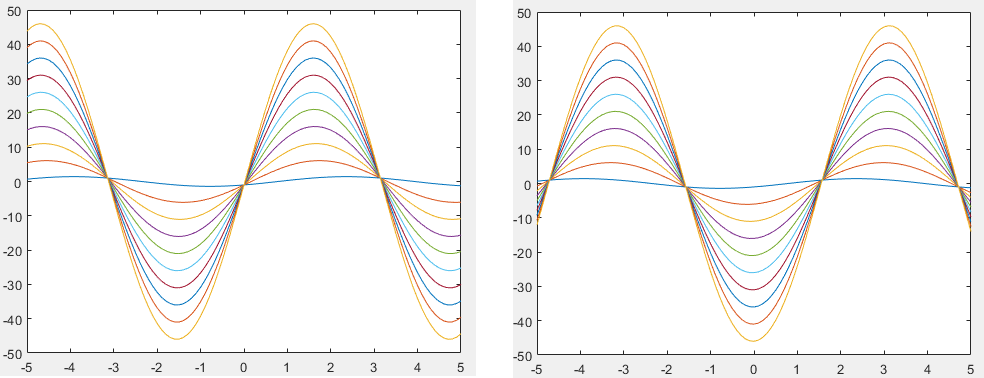
\includegraphics[width=1.0\textwidth]{assets/ht.PNG}
        \caption{Effect of changing (x,y) values to resulting sinusoid}
        \label{fig:hough_transform}
    \end{center}
\end{figure}


%%%%%%%%%%%%%%%%%%%%%%%%%%%%%%%%%%%%%%%%%%%%%%
% Q4
%%%%%%%%%%%%%%%%%%%%%%%%%%%%%%%%%%%%%%%%%%%%%%
\section{Impulse Response [5 pts]}
The Dirac delta function is a function that is 0 everywhere except in a very small part in the middle, there is a spike so big that the area under this spike is exactly 1.
The Dirac delta function is the identity value of the convolution operation, which means convolution with the dirac delta functions results in the original function, just like multiplying by 1 or adding 0 for real numbers. It does not change the original.

As a convolution kernel, the dirac delta function is an NxN matrix filled with 0 everywhere except a 1 in the middle. So it is clear that the value in the middle will be weighted 100\%, whereas every other value in an iteration has a weight of 0\% which means the value just stays the same.


src: http://math.stackexchange.com/questions/1015498/convolution-with-delta-function

src: https://de.wikipedia.org/wiki/Faltungsmatrix


%%%%%%%%%%%%%%%%%%%%%%%%%%%%%%%%%%%%%%%%%%%%%%
% Q4
%%%%%%%%%%%%%%%%%%%%%%%%%%%%%%%%%%%%%%%%%%%%%%
\section{Hough Transform for Line Detection [65 pts]}
\subsection{Edge Detection [20 pts]}
Non maximal supprssion is implemented by iterating through every pixel in the magnitude image and comparing the current pixel to the pixel above and below (left and right respectively). If the current pixel is not the biggest of the three, the pixel is set to 0 to suppress it and make the edge thinner and more accurate.

\begin{lstlisting}
% non maximal suppression
[width, height] = size(Iconv);
for x = 1:width
    for y = 1:height
        p = Im(x, y); % current pixel
        if (x > 1 && x < width) %a void index out of bounds
            if (p < Im(x-1, y) || p < Im(x+1, y))
                Im(x, y) = 0;
            end
        end
        if (y > 1 && y < height) %a void index out of bounds
            if (p < Im(x, y-1) || p < Im(x, y+1))
                Im(x, y) = 0;
            end
        end
    end
end
\end{lstlisting}







Fill your answers.

You can insert your figure by using \verb|\begin{figure}|.
You can refer your figure by using \verb|\ref{fig:example_figure}|.

\begin{figure}[!h]
    \begin{center}
        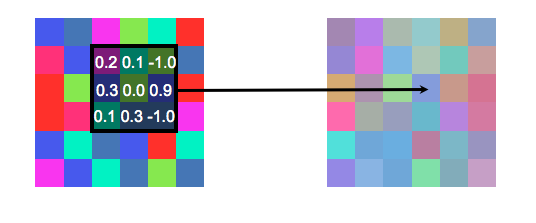
\includegraphics[width=0.7\textwidth]{assets/fig1.png}
        \caption{Example Figure}
        \label{fig:example_figure}
    \end{center}
\end{figure}

You can enumerate subquestions like this.

\begin{enumerate}
    \item Enumerate item 1.
    \item Enumerate item 2.
    \item Enumerate item 3.
\end{enumerate}

You can write your equations by using \verb|\begin{aligned}|.
We highly recommend you to use \verb|\newcommand| to simplify your equation in \LaTeX.

\begin{align}
    \Ab &= 12 \\
    \alpha_{12}^{35} &= 1234 \\
    \beta_1 &= 10
\end{align}

You can cite your reference by using \verb|\cite{reference_name}|.
For example, cite R.Szeliski's Compute Vision book \cite{szeliski2010computer} like this.


src: 
https://en.wikipedia.org/wiki/Canny_edge_detector


%%%%%%%%%%%%%%%%%%%%%%%%%%%%%%%%%%%%%%%%%%%%%%
% Q2
%%%%%%%%%%%%%%%%%%%%%%%%%%%%%%%%%%%%%%%%%%%%%%
\section{Some materials for HW2 [5 points]}

\begin{table}[!h]
\centering
\begin{tabular}{c|l|l|l|l}
Step & \multicolumn{1}{c|}{\begin{tabular}[c]{@{}c@{}}Variable\\ eliminated\end{tabular}} & \multicolumn{1}{c|}{\begin{tabular}[c]{@{}c@{}}Factors\\ used\end{tabular}} & \multicolumn{1}{c|}{\begin{tabular}[c]{@{}c@{}}Variables\\ involved\end{tabular}} & \multicolumn{1}{c}{\begin{tabular}[c]{@{}c@{}}New\\ factor\end{tabular}} \\ \hline
1    &                                                                                    &                                                                             &                                                                                   &                                                                          \\
2    &                                                                                    &                                                                             &                                                                                   &                                                                          \\
3    &                                                                                    &                                                                             &                                                                                   &                                                                          \\
4    &                                                                                    &                                                                             &                                                                                   &                                                                          \\
5    &                                                                                    &                                                                             &                                                                                   &                                                                          \\
6    &                                                                                    &                                                                             &                                                                                   &                                                                          \\
7    &                                                                                    &                                                                             &                                                                                   &                                                                         
\end{tabular}
\caption{A run of variable elimination for the query $P(J)$}
\label{table:VE}
\end{table}

% Bibtex
\bibliography{writeup}
\bibliographystyle{plain}

\end{document}
